\documentclass[10pt]{article}
\usepackage[cp1251]{inputenc}
\usepackage[english]{babel}
\usepackage{graphicx}
\usepackage[mag=1000,a4paper,left=2.2cm,right=3.0cm,top=3.0cm,bottom=3.0cm]{geometry}
\usepackage{enumerate}

\usepackage{latexsym, amsgen, amsmath, amstext, amsbsy, amsopn, amsfonts, amsthm, amssymb, amscd}
\usepackage{mathtext}
\usepackage{mathrsfs}

\title{Advanced Robotics}
\author{Melnikov E.\,R., Markeeva L.\,B., Usvyatsov M.\,R.}
\usepackage[cp1251]{inputenc}
\usepackage[normalem]{ulem}
\usepackage{indentfirst}
\usepackage{grffile}
\usepackage{epstopdf}
\usepackage{makeidx}
\usepackage{verbatim}
\usepackage{tikz}
\usepackage{ulem}
\usetikzlibrary{arrows}
\usetikzlibrary{shapes}
\usetikzlibrary{positioning}
\usetikzlibrary{calc}
\usepackage{caption}
\usepackage{hyperref}
\graphicspath{{images/}}

\frenchspacing
\parindent=0.6cm
\parskip=2pt
\mathsurround=1pt

\sloppy
\newtheorem{df}{Definition}
\newtheorem{stmt}{Statement}

\newtheorem{notice}{Notice}
\newtheorem{theo}{Theorem}

\def\proof{{\indent Proof.}}


\newcommand{\itemi}[1]{\item \emph{#1} }

\begin{document}
	\maketitle
	\section{Question 2}
		\begin{equation}
			L_1(a, b) = |a_x - b_x| + |a_y - b_y|
		\end{equation}
		
		\begin{equation}
			L_2(a, b) = \sqrt{(a_x - b_x)^2 + (a_y - b_y)^2}
		\end{equation}
		
		\begin{equation}
			L_{\infty} (a, b) = \max \left\{|a_x - b_x|, |a_y- b_y||\right\}
		\end{equation}
		
		8-connected distance equals to $L_{\infty}$ \cite{morse1998lecture}
		
		Hence: 
		\begin{equation}
			L_1(S, T_1) = 10
		\end{equation}
		
		\begin{equation}
			L_1(S, T_2) = 8
		\end{equation}
		
		\begin{equation}
			L_1(S, T_3) = 16
		\end{equation}
		
		\begin{equation}
			L_2(S, T_1) = \sqrt{68}
		\end{equation}
		
		\begin{equation}
			L_2(S, T_2) = \sqrt{40}
		\end{equation}
		
		\begin{equation}
			L_2(S, T_3) = \sqrt{136}
		\end{equation}
		
		\begin{equation}
			L_3(S, T_1) = 8
		\end{equation}
		
		\begin{equation}
			L_3(S, T_2) = 6
		\end{equation}
		
		\begin{equation}
			L_3(S, T_3) = 10
		\end{equation}
		
		Thus, in all distance metrics the closest one to S id $T_2$
	\newpage
	\section{Question 3}
		\subsection{Visibility graph}
			\begin{figure}[h!]
				\center{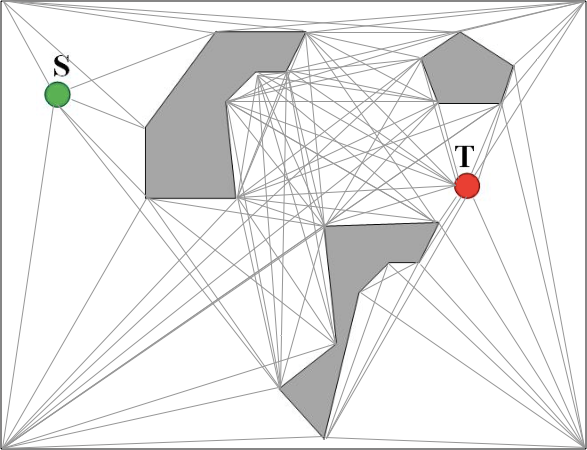
\includegraphics[width=0.7\textwidth]{1}}
				\caption{Visibility graph}
				\label{fig:modules}
			\end{figure}
		\subsection{Tangent graph}
			\begin{figure}[h!]
				\center{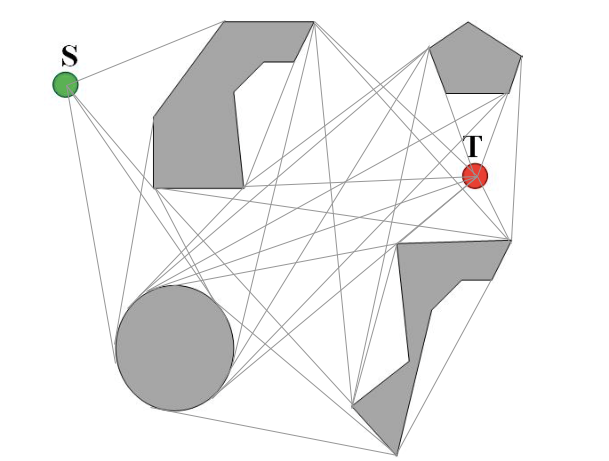
\includegraphics[width=0.7\textwidth]{2}}
				\caption{Tangent graph}
				\label{fig:modules1}
			\end{figure}
		\newpage
	\begin{thebibliography}{1}
		\bibitem{morse1998lecture} Morse, S Bryan, \emph{Lecture 2: Image Processing Review, Neighbors, Connected Components, and Distance}, Bringham Young University, 1998, pp. 6--7
	\end{thebibliography}
\end{document}
